\subsection{Sistema adaptado a todos os dispositivos}
Hoje em dia, o acesso à aplicações \textit{web} através de dispositivos móveis é cada vez maior.

A garantia de uma maior experiência de visualização, fácil leitura e a redução do redimensionamento do conteúdo da aplicação são fatores que contribuem para o sucesso da mesma.

Esses mesmos fatores foram tidos em consideração nesta aplicação, garantindo que esta está preparada para ser acedida em dispositivos de diferentes resoluções.

Nas imagens seguintes são representadas algumas das principais páginas da aplicação quando visionadas em ecrãs de menor resolução:

\begin{figure}[H]
	\centering
 	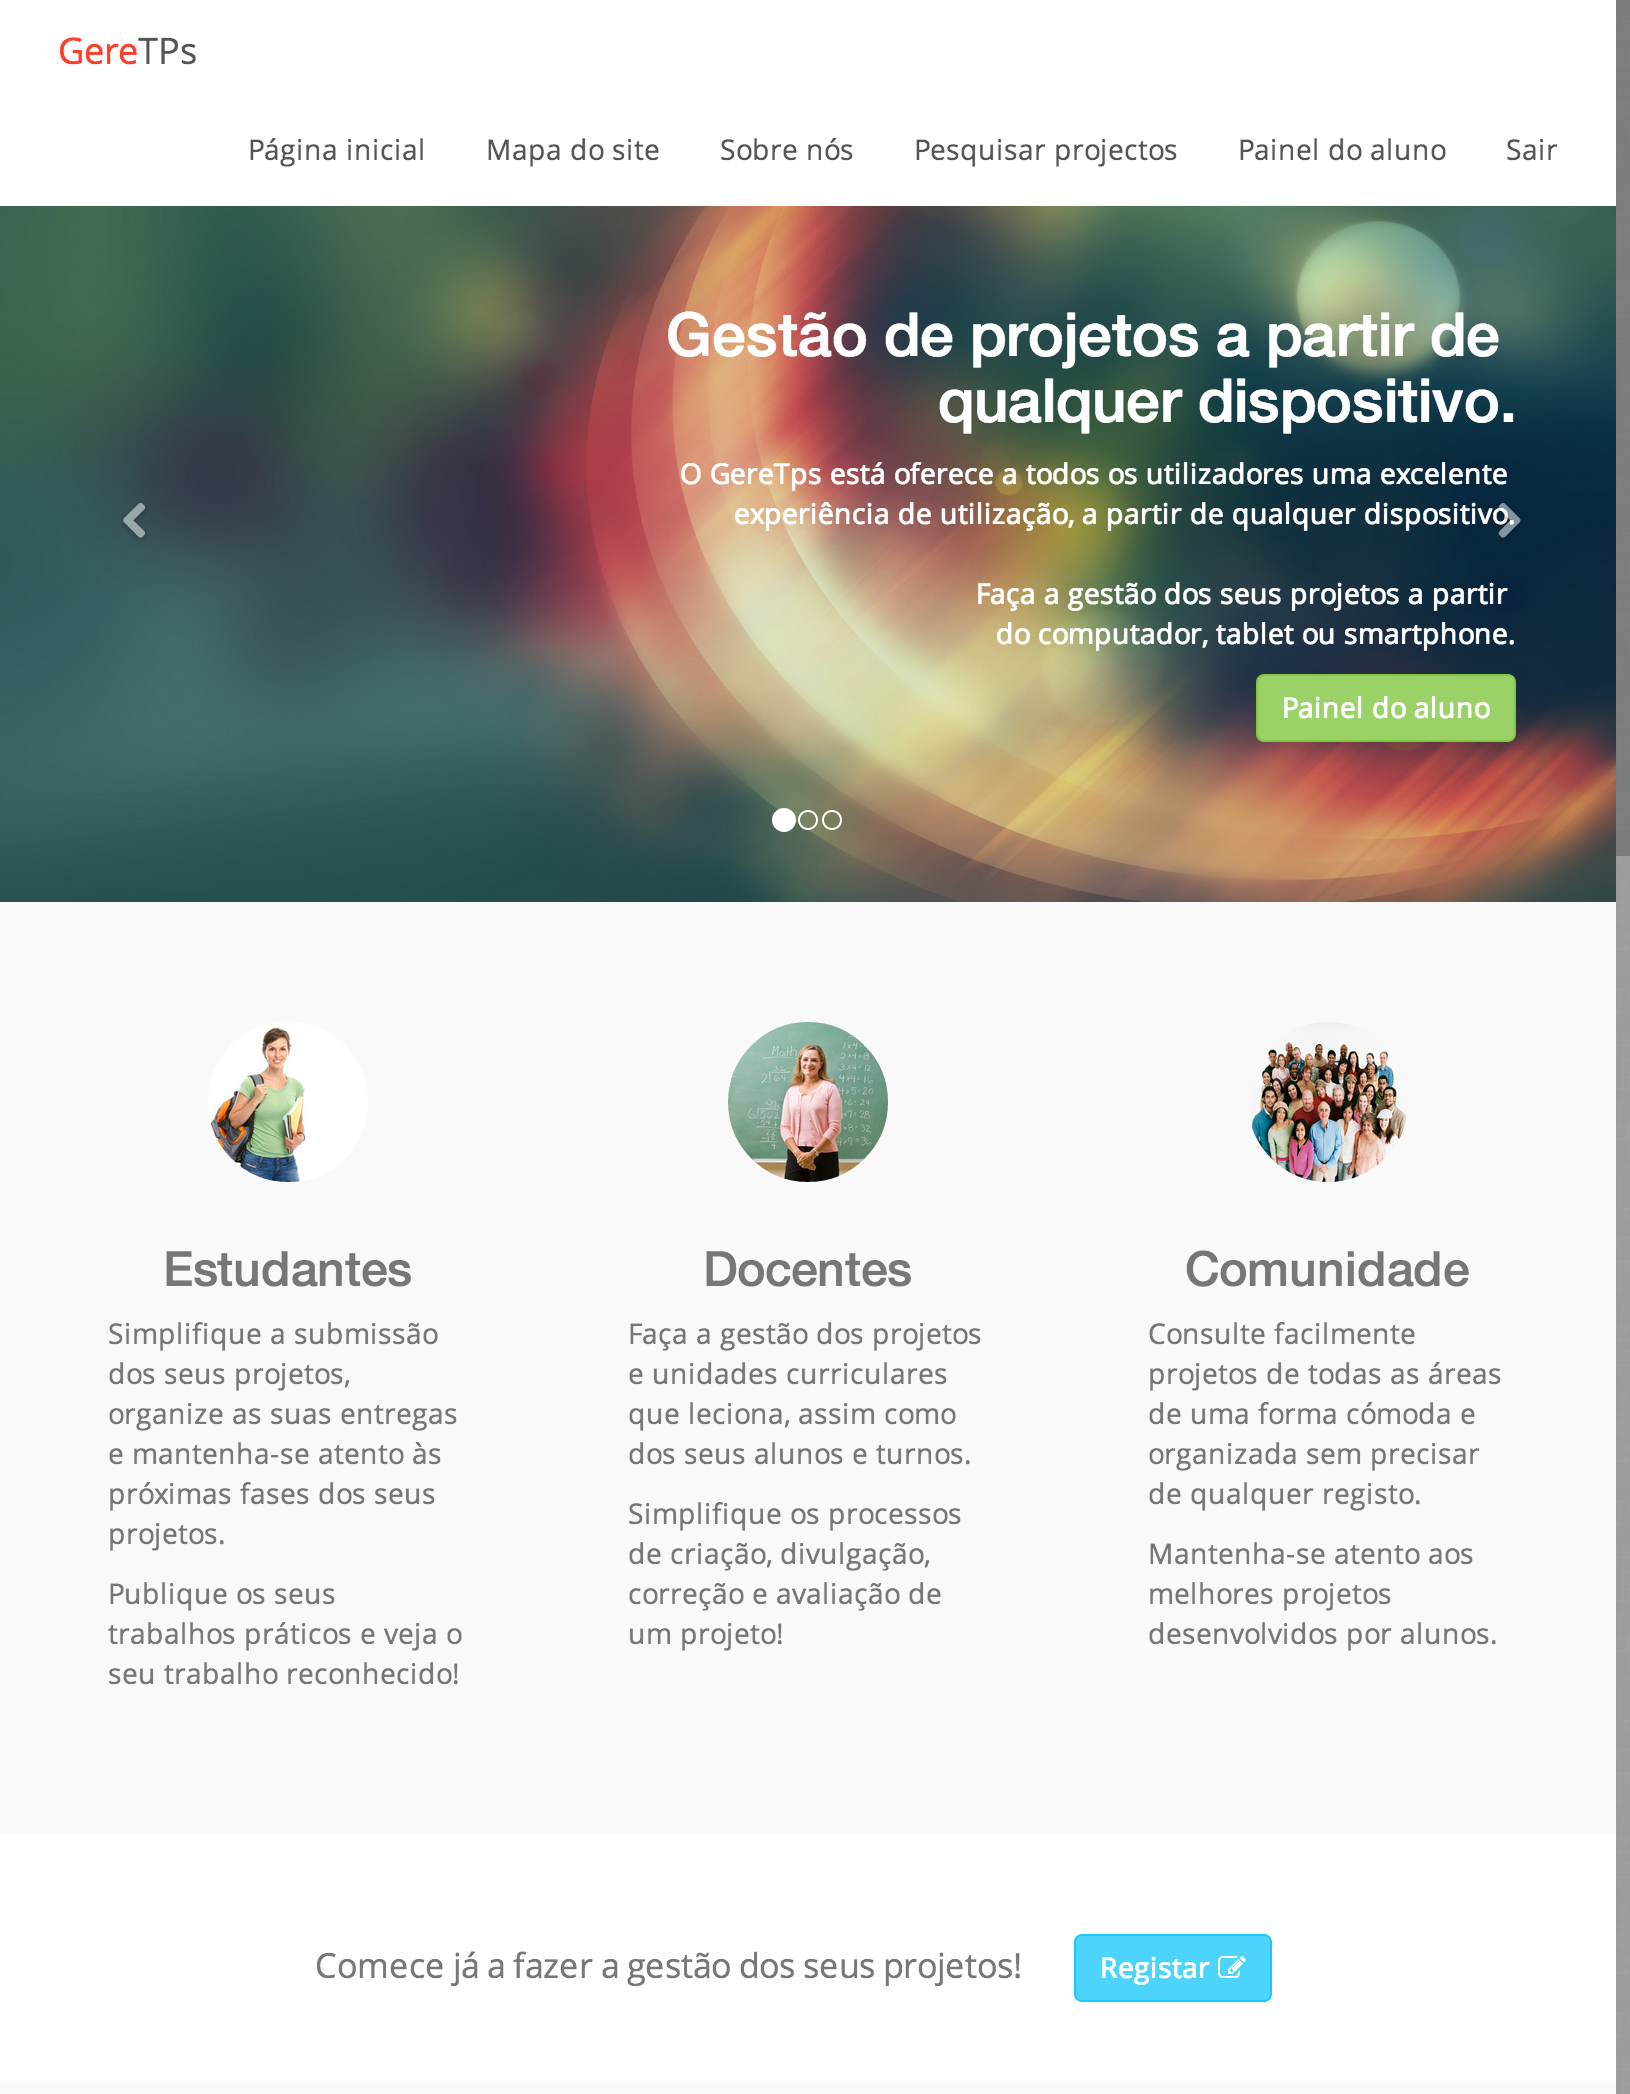
\includegraphics[width=0.65\textwidth,center]{images/implementacao/alunos/home}
 	\caption{Página Inicial}
 	\label{fig:home_smal}
 \end{figure}

\begin{figure}[H]
	\centering
	\begin{subfigure}{0.5\textwidth}
 		\centering
 		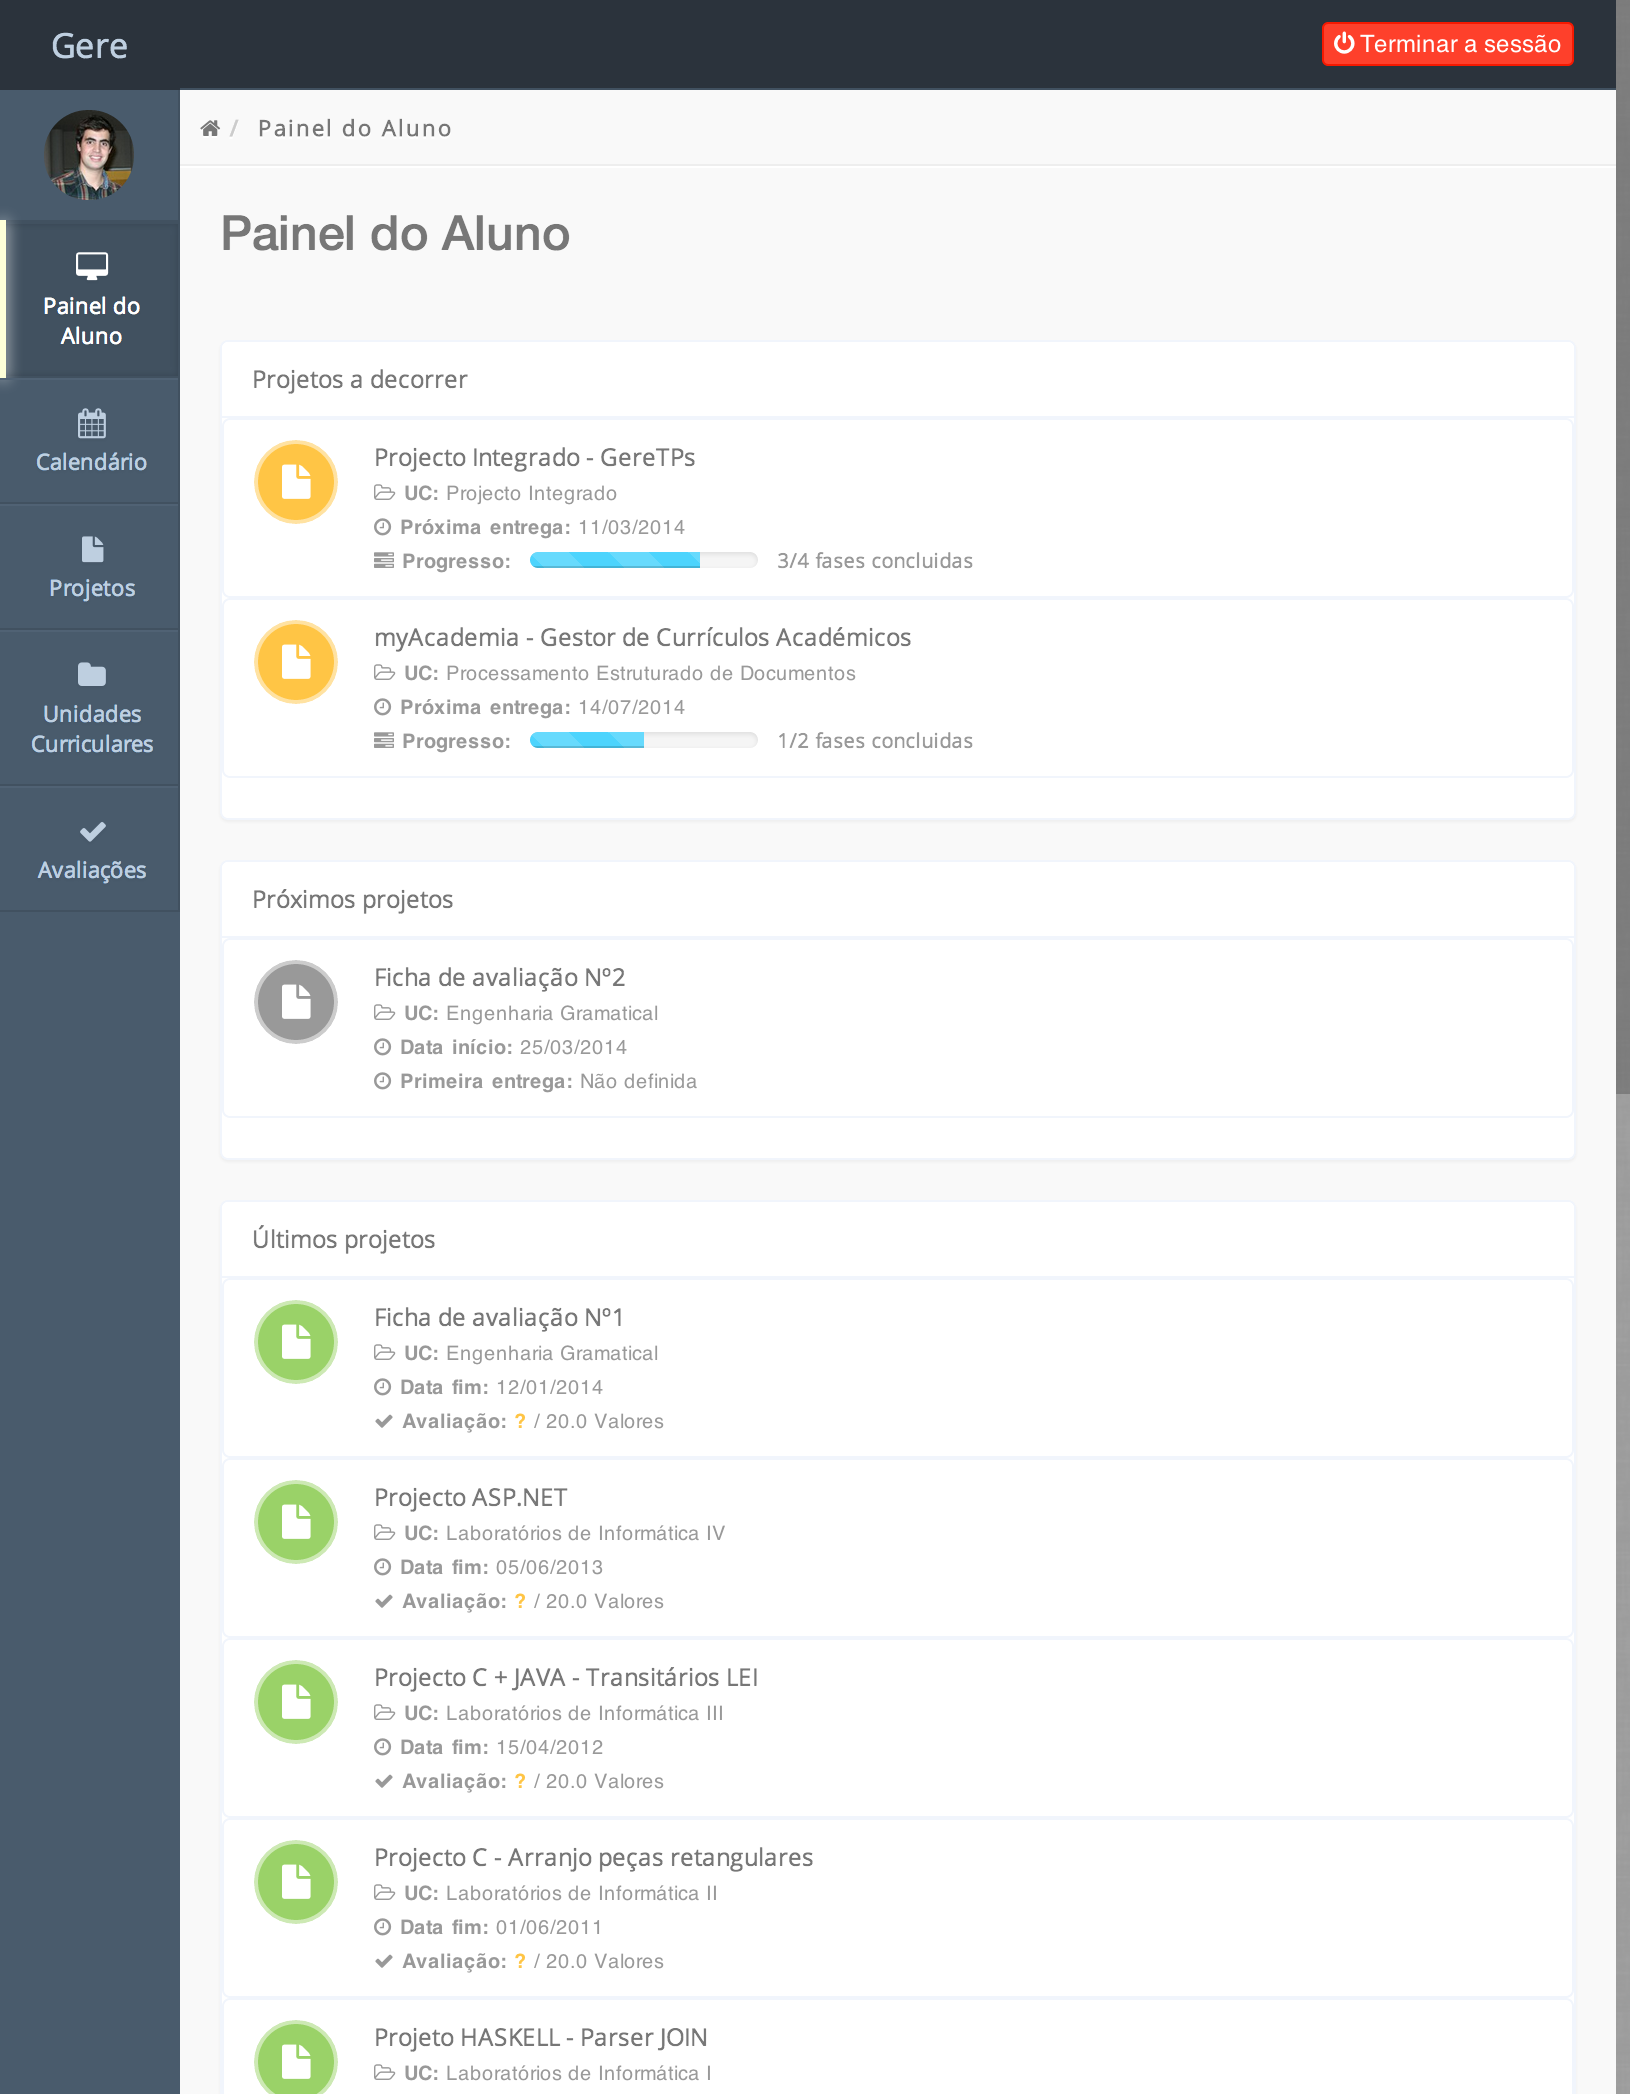
\includegraphics[width=0.95\textwidth,center]{images/implementacao/alunos/dashboard_small}
 		\subcaption{Painel do aluno}
 		\label{fig:dashboard_small}
 	\end{subfigure}
 	\begin{subfigure}{0.55\textwidth}
	 	\centering
	 	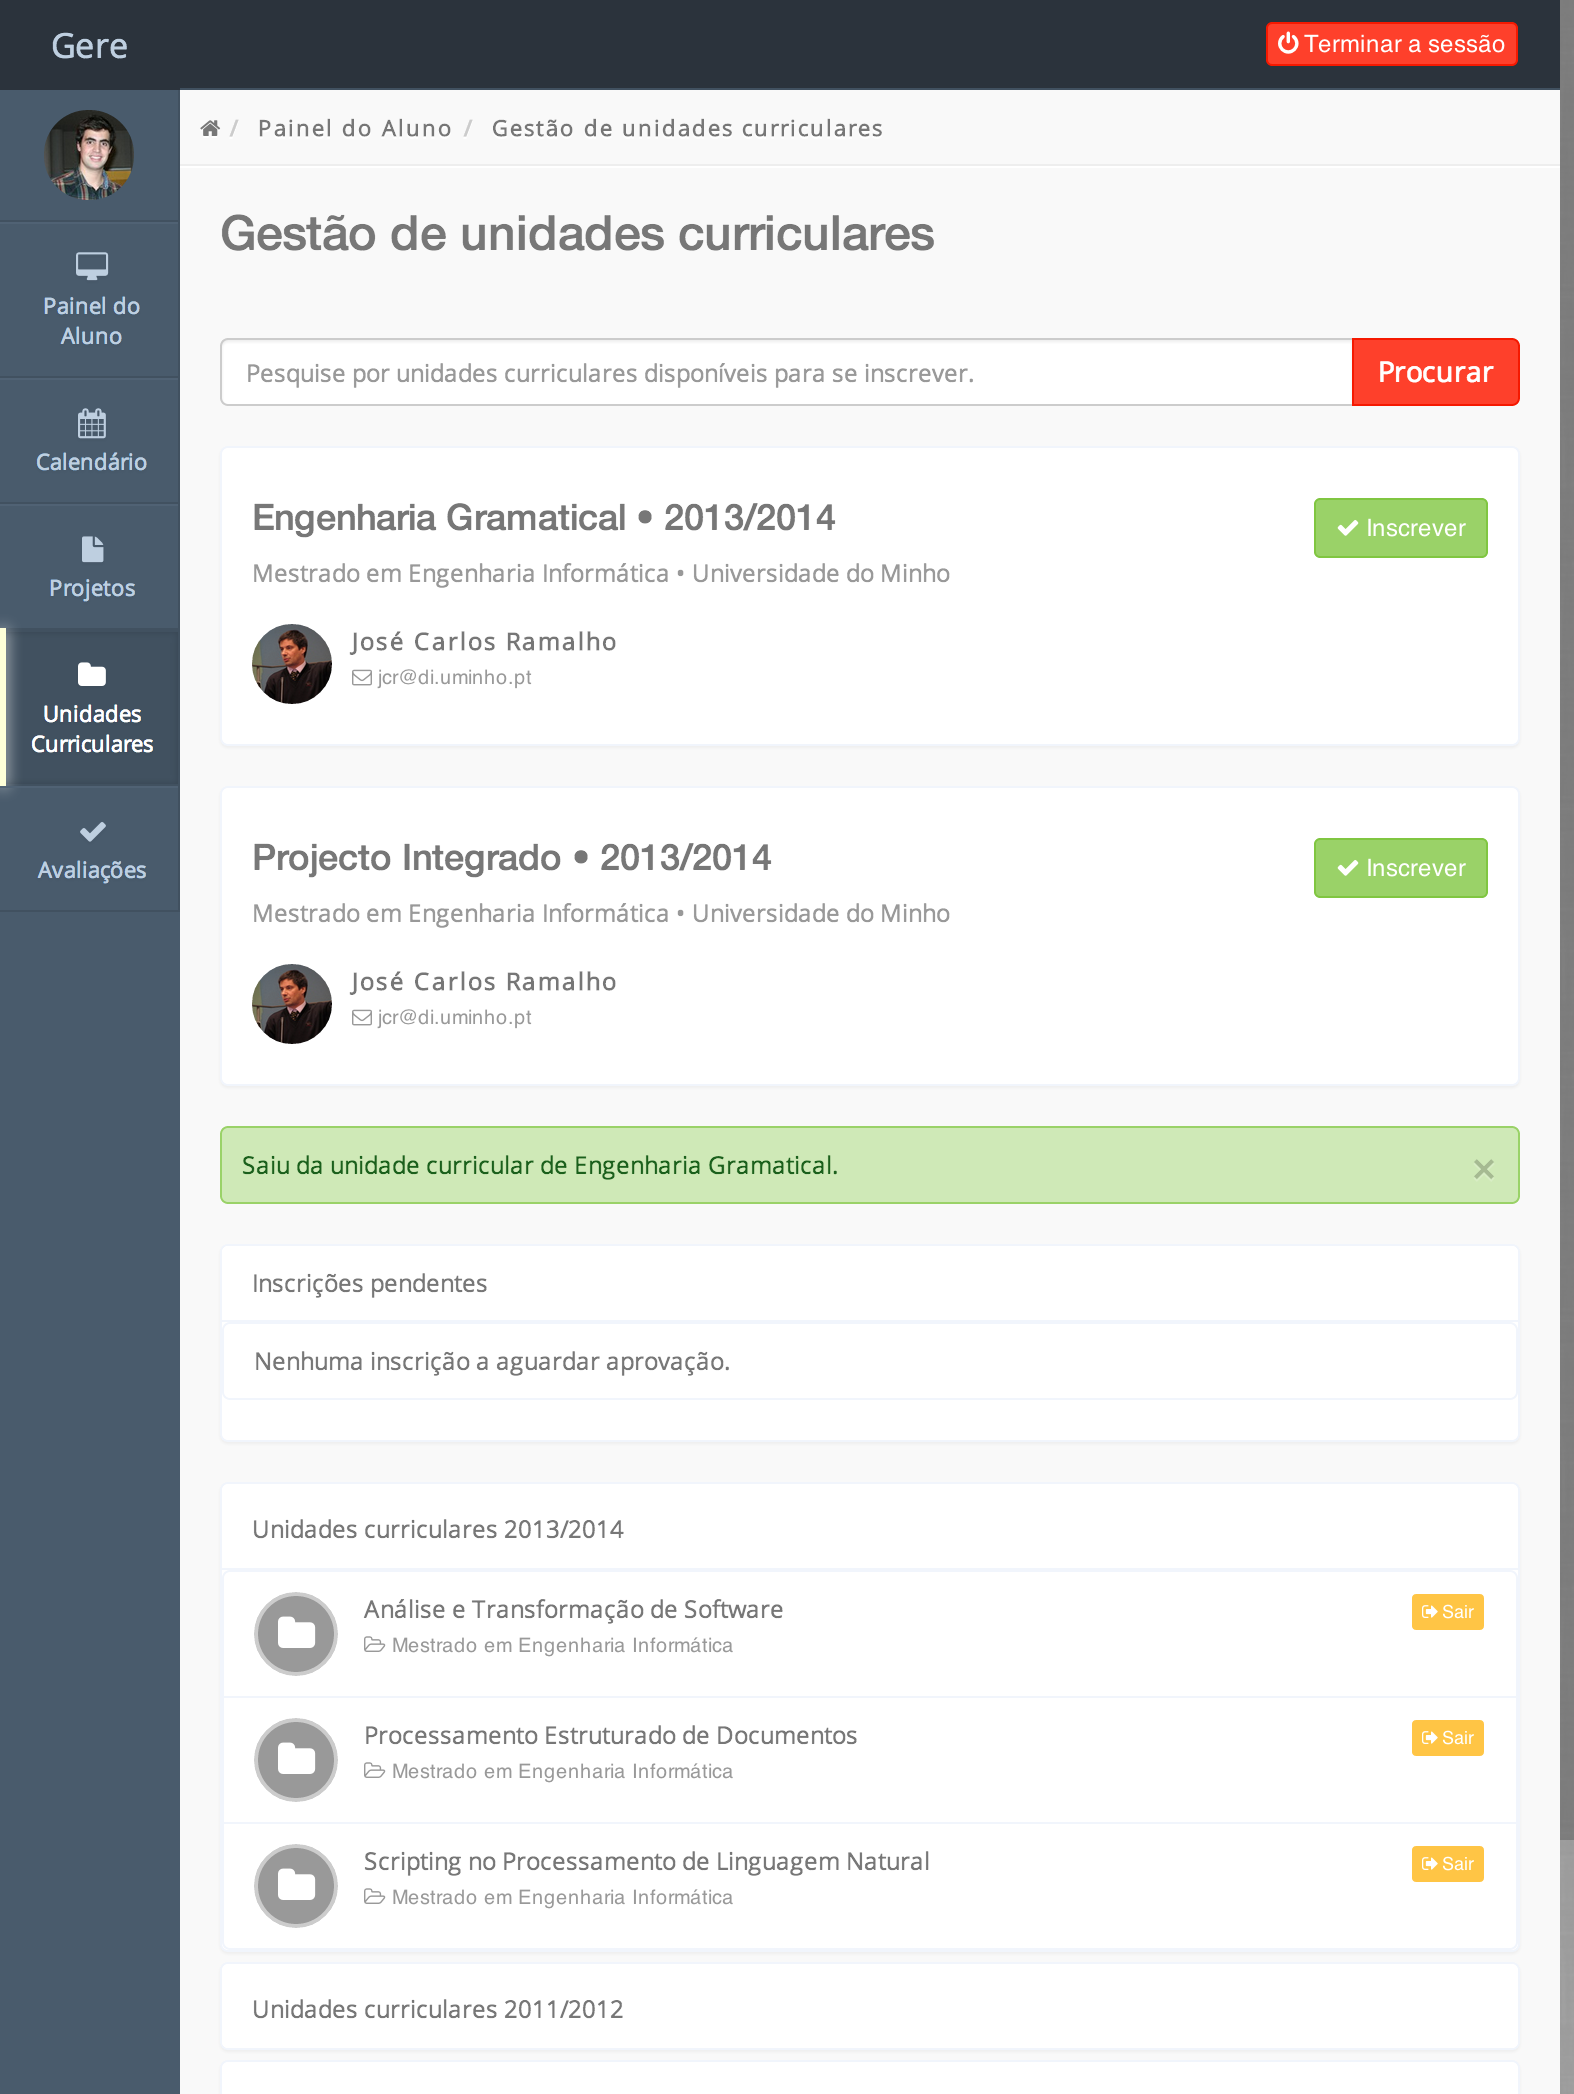
\includegraphics[width=0.95\textwidth,center]{images/implementacao/alunos/ucs}
	 	\subcaption{Gestão de unidades curriculares}
	 	\label{fig:ucs_small}
 	\end{subfigure}
 \end{figure}


 \begin{figure}[H]
	\centering
	\begin{subfigure}{0.45\textwidth}
 		\centering
 		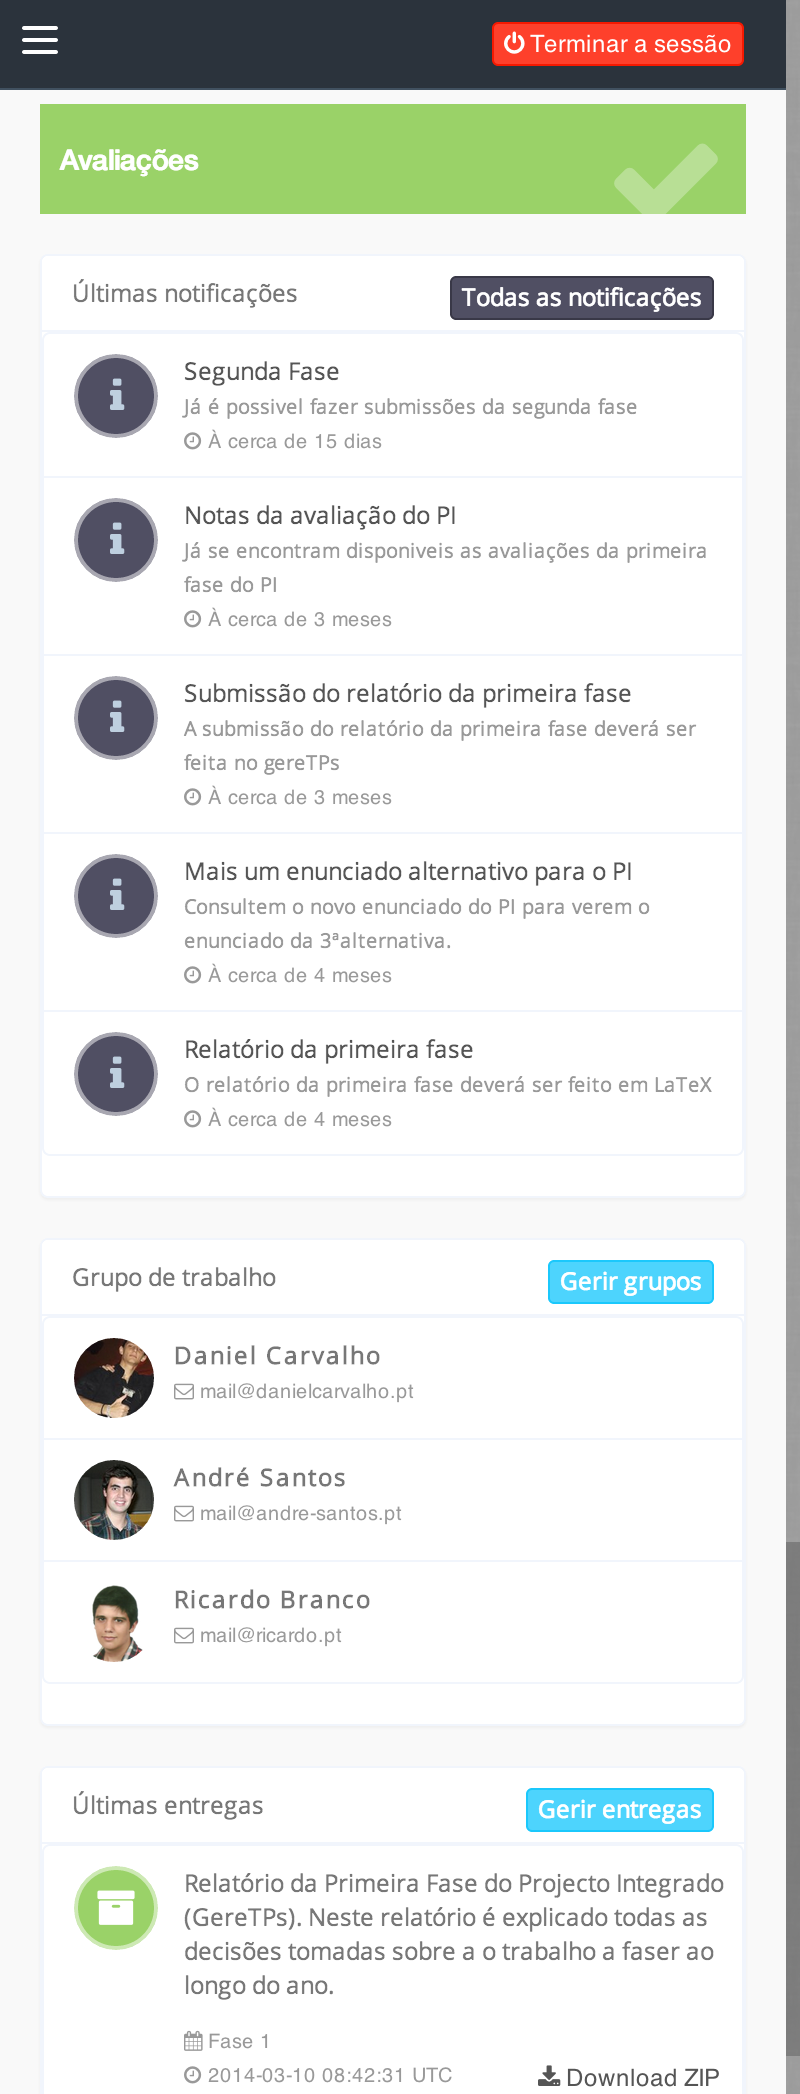
\includegraphics[width=0.95\textwidth]{images/implementacao/alunos/project_small}
 		\subcaption{Página de um projeto}
 		\label{fig:project_small}
 	\end{subfigure}
 	\begin{subfigure}{0.45\textwidth}
 		\centering
 		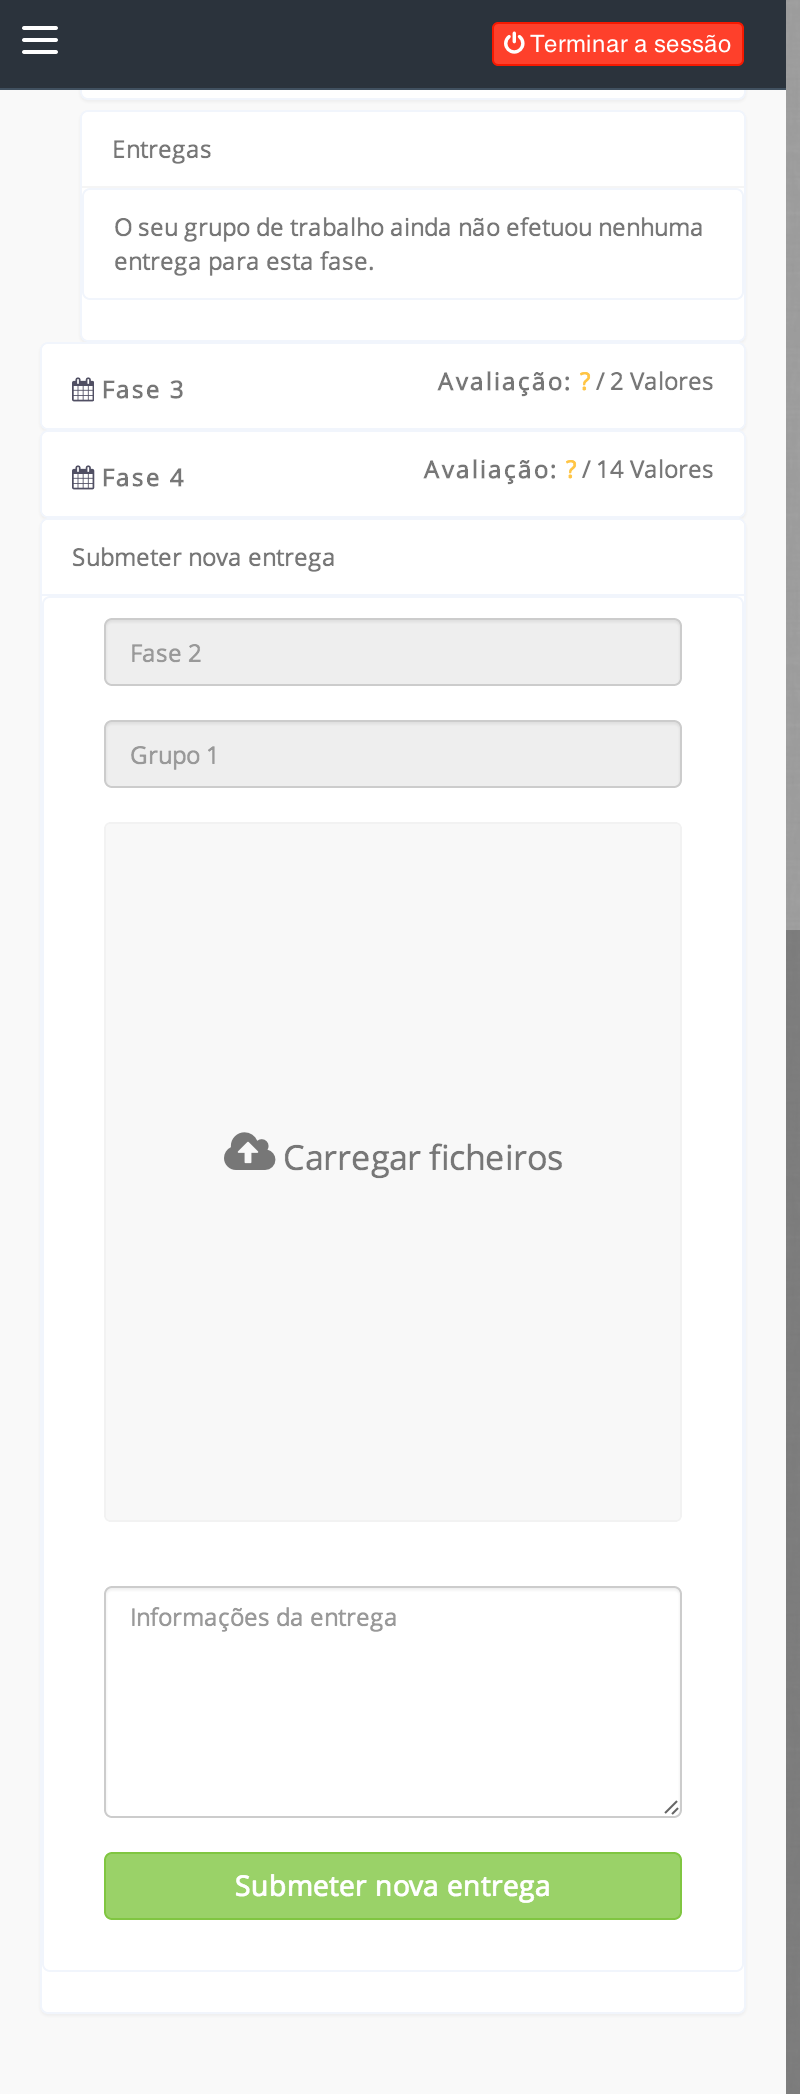
\includegraphics[width=0.95\textwidth]{images/implementacao/alunos/entrega}
 		\subcaption{Entrega de uma fase}
 		\label{fig:delivery_small}
 	\end{subfigure}
 \end{figure}




